% Graph Theory Assignments
% Declare overall type of document (use 11pt report class on A4 paper).
\documentclass[11pt,a4paper]{report}

% Include the style file which contains all the required formatting
% information that is set out in the Research Higher Degrees Resource
% Handbook (2003 version). NOTE: This file uses the following packages
% 'graphicx' for graphics manipulation
% 'fancyhdr' for nice headers and footers.
% 'makeidx' for generating the index
% 'tocbibind' for adding table of contents entries for bibliography, index etc.
% 'sectsty' for generating stylised chapter and section headings.
% You will need to make sure your LaTeX installation has these packages
% installed...else it wont work :(
\usepackage{enumerate}
\usepackage{MathPhysHonoursThesis}
\usepackage{float}
\usepackage{tikz}
\usetikzlibrary{positioning}
\usetikzlibrary{arrows}

% Need this to get rid of annoying error
%\pgfplotsset{compat=1.12}

%% newcommands.tex (new command definitions)

% Here you would include any additional packages that you want to use.
% You should make sure they don't clash with the above packages that
% are in use in the style file.
% If you want to call in some style files or new packages, put them here
\usepackage{undertilde}
%\usepackage[left=2cm,right=2cm,top=2cm,bottom=2cm]{geometry}
\usepackage[a4paper]{geometry}
\usepackage[latin1]{inputenc}
\usepackage{amsmath, latexsym, color, graphicx, amssymb, here}
\usepackage{amsfonts}
\usepackage{epsf, epsfig, pifont,tikz}
\usepackage{graphics, calrsfs}
%\usepackage{tangocolors}
\usepackage{times}
\usepackage{fancybox,calc}
\usepackage{hyperref}
\usepackage{pgfplots}
\usepackage{verbatim}

% Some examples (yours may be different):
\newtheorem{theorem}{Theorem}[section]
\newtheorem{lemma}[theorem]{Lemma}
\newcommand{\bfx}{{\ensuremath{\mathbf{x}}}}

\newcommand{\A}{{\bf A}}
\newcommand{\B}{{\bf B}}
\newcommand{\T}{{\bf T}}
\newcommand{\C}{{\bf C}}
\newcommand{\N}{{\bf N}}
\newcommand{\R}{{\mathbb R}}
\newcommand{\Z}{{\mathbb Z}}
\newcommand{\n}{{\bf n}}
\renewcommand{\v}{{\bf v}}
\renewcommand{\r}{{\bf r}}
\renewcommand{\a}{{\bf a}}

\newcommand{\uniti}{{\hat{\mbox{\boldmath $\imath$}}}}
\newcommand{\unitj}{{\hat{\mbox{\boldmath $\jmath$}}}}
\newcommand{\unitk}{{\hat{\mbox{\boldmath $\mathit{k}$}}}}
\newcommand{\unitn}{{\hat{\mbox{\boldmath $\mathit{n}$}}}}
\newcommand{\unite}{{\hat{\mbox{\boldmath $\mathit{e}$}}}}
\newcommand{\unitu}{{\hat{\mbox{\boldmath $\mathit{u}$}}}}
\newcommand{\ie}{{\em i.e.} \/}
\newcommand{\eg}{{\em e.g.} \/}
\newcommand{\etc}{{\em etc.} \/}
\newcommand{\etal}{{\em et al. }}
\newcommand{\mathbi}[1]{\textbf{\em #1}}
\newcommand{\bcdot}{\mbox{\boldmath $\, \cdot \, $}}
\newcommand{\vect}[1]{{\mbox{\boldmath $\utilde{\mathit{#1}}$}}}
\newcommand{\xyplane}{$x$-$y$ plane \/}
\newcommand{\xzplane}{$x$-$z$ plane \/}
\newcommand{\yzplane}{$y$-$z$ plane \/}
\newcommand{\dint}{\int \! \! \int}
\newcommand{\tint}{\int \! \! \int \! \! \int}
\newcommand{\doint}{\bigcirc \! \! \! \! \! \! \! \! \int \! \! \! \! \!  \int}
\newcommand{\inlinedoint}{\circ\!\!\!\! \! \int \!\!\!\! \int}
%\newcommand{\deloperator}[3]{{\frac{\partial{#1}}{\partial x} \, \uniti \frac{\partial{#2}}{\partial y} \, \unitj + \frac{\partial{#3}}{\partial z} \, \unitk}}
\newcommand{\deloperator}{{\frac{\partial}{\partial x} \, \uniti + \frac{\partial}{\partial y} \, \unitj + \frac{\partial}{\partial z} \, \unitk}}
\newcommand{\laplaceoperator}{{\frac{\partial^2}{\partial x^2} + \frac{\partial^2}{\partial y^2} + \frac{\partial^2}{\partial z^2}}}
%\newcommand{\grad}[1]{{\frac{\partial {#1}}{\partial x} \, \uniti + \frac{\partial {#1}}{\partial y} \, \unitj + \frac{\partial {#1}}{\partial z} \, \unitk}}
\newcommand{\gradCylindrical}[1]{{\frac{\partial {#1}}{\partial \rho} \, \unite_\rho \ + \ \frac{1}{\rho} \frac{\partial {#1}}{\partial \phi} \, \unite_\phi \ + \ \frac{\partial {#1}}{\partial z} \, \unite_z} }
\newcommand{\gradSpherical}[1]{{\frac{\partial {#1}}{\partial r} \, \unite_r \ + \ \frac{1}{r} \frac{\partial {#1}}{\partial \theta} \, \unite_\theta \ + \ \frac{1}{r \sin(\theta)}\frac{\partial {#1}}{\partial \phi} \, \unite_\phi} }
\newcommand{\divSpherical}[3]{{\frac{1}{R^2}\, \frac{\partial}{\partial R}\left(R^2\, {#1}\right) \ + \  \frac{1}{R \sin(\theta)} \frac{\partial}{\partial \theta} \left(\sin(\theta)\, {#2}\right) \ + \ \frac{1}{R \sin(\theta)}\frac{\partial {#3}}{\partial \phi} \  }}
%\newcommand{\laplacian}[1]{{\frac{\partial^2 {#1}}{\partial x^2} + \frac{\partial^2 {#1}}{\partial y^2} + \frac{\partial^2 {#1}}{\partial z^2}}}
\newcommand{\posvect}[1]{{#1}_1 \, \uniti + {#1}_2 \, \unitj + {#1}_3 \, \unitk}
\newcommand{\posvectr}{x \, \uniti + y \, \unitj + z \, \unitk}
\newcommand{\posvectcyl}{\rho \, \unite_\rho \, + z \, \unite_z}
\newcommand{\posvectsph}{r \, \unite_\r}
\newcommand{\arbvect}[3]{{#1} \, \uniti \, + \, {#2} \, \unitj \, + \, {#3} \, \unitk}
\newcommand{\genvect}[5]{{#1} \, \uniti \, {#2}\,  {#3} \, \unitj \, {#4} \, {#5} \, \unitk}
\newcommand{\parametricposvectr}{\vect{r}(t) \ = \ x(t) \, \uniti + y(t) \, \unitj + z(t) \, \unitk}
\newcommand{\divergence}[1]{\nabla \bcdot \vect{#1}}
%\newcommand{\curl}[1]{\nabla \times \vect{#1}}
\newcommand{\magnitude}[1]{ \| \vect{#1} \| }
\newcommand{\drCart}{d x \, \uniti + d y \, \unitj + d z \, \unitk}
\newcommand{\drCyl}{d \rho \, \unite_\rho + \rho \, d \phi \, \unite_\phi + d z \, \unite_z}
\newcommand{\drSph}{d r \, \unite_r + r \, d \theta \, \unite_\theta + r \, \sin(\theta) \, d \phi \, \unite_\phi }
\newcommand{\coordvect}[3]{{#1} \, \uniti \, + \, {#2} \, \unitj \, + {#3} \, \unitk}
\newcommand{\cylcoordvect}[3]{{#1} \, \unite_\rho \, + \, {#2} \, \unite_\phi \, + {#3} \, \unite_z}
\newcommand{\sphcoordvect}[3]{{#1} \, \unite_\r \, + \, {#2} \, \unite_\theta \, + {#3} \, \unite_\phi}

\newcommand{\ul}[1]{\underline{#1}}

\newsavebox{\fmbox}
\newenvironment{eqnframe}[1]     
{
	\begin{center} 
	\begin{lrbox}{\fmbox}
	\begin{minipage}{#1}
}     
{
	\end{minipage}
	\end{lrbox}\fbox{\usebox{\fmbox}}
	\end{center}
}

\newcommand\Tpad{\rule[4.5ex]{0pt}{0pt}}
\newcommand\Bpad{\rule[-3.75ex]{0pt}{0pt}}

\renewcommand{\labelenumi}{\textbf{\arabic{enumi}}.}
\renewcommand{\labelenumii}{\textbf{(\roman{enumii})}}
\renewcommand{\labelenumiii}{\textbf{(\alph{enumiii})}}

\newcommand{\parD}[2]{\frac{\partial #1}{\partial #2}}
\newcommand{\parDD}[2]{\frac{\partial^2 #1}{\partial #2 ^2}}
\newcommand{\laplacian}{\Delta}
\renewcommand{\div}{\nabla\cdot}
\newcommand{\grad}{\nabla}
\newcommand{\divp}{\nabla^\prime\cdot}
\newcommand{\gradp}{\nabla^\prime}
\newcommand{\curl}{\nabla\times}
\newcommand{\cross}{\times}
\renewcommand{\dot}{\cdot}
% define some colors
\definecolor{cBlue}{rgb}{.255,.41,.884} % RoyalBlue of svgnames
\definecolor{cRed}{rgb}{1, 0, 0} % Red of svgnames



\includeonly{
chap1  % Assignment Questions Week 1
,chap2  % Week 2
,chap3  % Theory (Feature Extraction)
,chap4  % Theory (Classification)
,chap5	% Segmentation Techniques in Detail
,chap6	% How we compare
% ,chap7	% Results
% % ,chap8	% Conclusion/Discussion
% %,app0   % Needed to switch to appendix mode
% ,app1   % Tables and Figures
% ,app2   % R code
% % % ,app3   % Python code
% % % ,app4   % Glossary A
% % % ,app5   % Glossary B
% ,biby   % Makes the bibliography from the BibTeX database
}






\begin{document}

\pagenumbering{arabic}

% chap1.tex (Week 1 questions)

% Note that the text in the [] brackets is the one that will
% appear in the table of contents, whilst the text in the {}
% brackets will appear in the main thesis.

\chapter[Week 1]{Week 1}

\section{Q 1.2.9}

\begin{enumerate}[(a)]
\item I hate this question.
\item And this one too.
\end{enumerate}


\section{Q 1.3.1}

\begin{enumerate}[(a)]
\item By definition an edge is incident to 2 and only 2 vertices, thus the sum of objects incident to any edge is 2.

\item Without any restriction, the column sums of the adjancy matrix could take any value. For a simple graph the column sum has a maximum value of $v-1$ since there is a maximum of 1 edge to any vertex pair.
\end{enumerate}

\section{Q 1.6.8}

\begin{enumerate}[(a)]
\item Consider a single component graph. If one removes an edge from this graph there are two possible scenarios:\\
1. The edge is removed, but there is at least one other edge connecting any two disjoint subgraphs and so $\omega(G)$ does not change.\\
2. The edge was the only connection between two disjoint subgraphs and so the subgraphs become disconected and $\omega(G)$ increases by one. Since any edge can only connect two vertices, and thus only two subgraphs, it is not possible for the removal of an edge to increase $\omega(G)$ by more than one.\\
Any multi-component graph will act the same, as we can only take a single edge away from a single component at a time.


\item Removing a vertex can have a considerably larger effect than removing an edge. Consider the following two cases that break the equality:\\
1. We remove a vertex that is incident with no edges. In this case, the vertex makes up an entire disconnected component of its own, and so removing it removes a component; i.e. $\omega(G-v) \leq  \omega(G)$\\
2. We remove a vertex that is the only vertex shared by 3 different subgraphs:\\
Let $v$ be the vertex as described and $G_x$ be a subgraph containing $v$, $x = 0,1,2.$\\
Then we have  $G_0 \cap G_1 \cap G_2 = \{v\}$ \\
If we remove v then we have $G_0 \cap G_1 \cap G_2 = \emptyset$ \\
So we went from $\omega(G) = 1$ to $\omega(G) = 3$. Clearly $\omega(G-v) \geq \omega(G)+1$


\end{enumerate}


\section{Q 1.6.14}

\begin{enumerate}[(a)]
\item Let $G$ be simple, connected and incomplete. Consider 3 vertices $u, v,$ and $w$ with edges $uv, uw, vw \in E$   $\forall  u, v, w \in G$. Clearly each vertex in $G$ is connected to every other vertex in $G$ and so $G$ must be complete. This is a contradiction, to avoid the contradiction at least 1 of the possible set of three vertices must have the condition that at least 1 of $uv, uw, vw \notin E$
\end{enumerate}


\section{Q 1.7.2}
\begin{enumerate}[(a)]
\item Assume that $G$ is connected and acyclic. Therefore G is a tree, which means it must have $\delta = 1$. We have a contradiction and so G must contain a cycle.
\end{enumerate}


% Questions from week 2

\chapter[Week 2]{Week 2}

\section{Q 2.1.5}
\begin{enumerate}[(a)]
\item Since the number of edges of $G$ is constrained to $v-1$ we can construct any arbitrary connected graph by sequentially adding a vertex and edge pair to a kernel vertex. They must be added as a pair otherwise the \# edges constraint would be violated. Creating a cycle requires adding an edge between two vertices that already exist. Since we cannot at any stage do this, $G$ must be acyclic.\\
Since $G$ is connected and acyclic, it is a tree.

\item $G$ is acyclic and so it is a forest. Because it is a forest, we know that $\varepsilon(G) = v(G) - \omega(G)$ and we also have the condition that $\varepsilon(G) = v(G) - 1$. It is clear then that $\omega(G) = 1$ and therefore we have only 1 component which means that $G$ is connected.\\
Since $G$ is acyclic and connected, it is a tree.

\item $G$ is a tree which means it is acyclic and connected by definition.
\end{enumerate}


\section{Q 2.2.4}
\begin{enumerate}[(a)]
\item Since the textbook does not define a Maximal Forest, let's define it as follows:\\
$F$ is a maximal forest of $G$ when for every component $H$ of $G$, $F \cap H$ is a spanning tree of $H$.\\
Thus the solution is: by the definition above.

\item Each component of the forest is a tree with $v_{sub}-1$ edges where $\sum_{\omega}(v_{sub}) = v(G)$, so the total number of edges of the forest epsilon(F) is simply $\sum_{\omega}(v_{sub}) - \omega* 1$, i.e. $\varepsilon(F) = v(G) - \omega(G)$.
\end{enumerate}

\section{Q 2.2.6}
\begin{enumerate}[(a)]
\item Assuming that there IS a cut edge, imagine two disjoint subgraphs A and B of G s.t. there is only one edge e, not in A or B, connecting the two subgraphs, i.e. $A+B+e = G$. Now consider the vertex of $A$ that is the vertex in $G$ incident with $e$, since $e$ is not included in $A$, this vertex must have an odd degree $(even number - 1 = odd number)$. However, since every other vertex in $A$ must have an even degree, this is clearly (explain!) impossible so we have a contradiction.

\item Yuck. To be done.

\end{enumerate}

\section{Q 2.3.1}
\begin{enumerate}[(a)]
\item Clearly the cut edge must incident to two vertices, if we were to remove either of those vertices it would result in a loss of the edge as well. At a minimum such a cut vertex must increase the number of components by 1, but if it is also incident with other cut edges (which would also disappear) then correspondingly more components are created.

\item Consider a graph with a central node that is connected to all other vertices, and each pair of outer vertices is also connected. Such a graph has no cut edge but the central node is a cut vertex - removing it would increase the number of components drastically.

\end{enumerate}


% chap3.tex (Week 3 questions)

% Note that the text in the [] brackets is the one that will
% appear in the table of contents, whilst the text in the {}
% brackets will appear in the main thesis.

\chapter[Week 3 - Connectivity]{Week 3 - Connectivity}

\section{Q 3.1.2}
handshake lemma

\section{Q 3.1.6}

\section{Q 3.2.1}
Forwards: A 2-edge-connected graph must have $\delta \geq 2$. We have shown previously that any graph with $\delta \geq 2$ must have a cycle. This means that any subgraph of $G$ must contain a cycle, and so every vertex pair lies on a common cycle. It follows then that there is an edge disjoint path between every vertex in $G$
Backwards: $G$ has two edge-disjoint paths between any two vertices. This means every vertex pair must lie on a common cycle, and so you could remove any single edge from $G$ and it would still be connected. Thus 2-edge-connected.

\section{Q 3.2.6}
Hint: Form a new graph $G^\prime$ by adding two vertices $x$ and $y$, and joining $x$ to all vertices in $X$ and $y$ to all vertices in $Y$. Show that $G^\prime$ is 2-connected and apply theorem 3.2\\
Theorem 3.2: A graph G with $v \geq 3$ is 2-connectd if and only if any two vertices of $G$ are connected by at least two internally-disjoint paths.\\

Following the hint, we can say that $G^\prime = G + \{x\} + \{y\}$. Now, since $X$ and $Y$ must contain at least 2 vertices each, and $x$ and $y$ must be connected to every one of these vertices, in their respective sets, $d(x) \geq 2$ and $d(y) \geq 2$. There are three cases when we look for a cut vertex here:
\begin{itemize}
\item the cut vertex belongs to $G^\prime \cap G$, i.e. $G$, which is 2-connected. Hence $G^\prime \cap G$ remains connected, but what about $\{x\}$ and $\{y\}$? Since they have degree of at least two, and they are 2 edge-connected to $G$, they are thus 2-connected also and remain joined.
\item the cut vertex is $x$. $x$ is removed, leaving $G + \{y\}$ which is connected.
\item the cut vertex is $y$. Identical argument to the above.
\end{itemize}
So we are satisfied that $G^\prime$ is 2-connected.\\
We can now use Th. 3.2 to say that since $G^\prime$ is 2-connected there must exist two internally disjoint paths originating at $x$ and terminating at $y$, which we will define as 
\[
p = \{x_p, X_{p1}, X_{p2},\ldots,G_{p1},G_{p2},\ldots,Y_{p1},Y_{p2},\ldots, y\} 
\]
and 
\[
q = \{x_q, X_{q1}, X_{q2},\ldots,G_{q1},G_{q2},\ldots,Y_{q1},Y_{q2},\ldots, y\}. 
\]
Clearly we can remove end elements from this path until we have $G_{.1},\ldots,G{..}$ which gives two disjoint paths connecting $X$ and $Y$.

\section{Q 3.3.3}
Find a graph with 9 vertices, 23 edges, that is 5-connected but not isomorphic to the graph $H_{5,9}$ shown in the book.

Remove the edge 0,8 and add in new edge 8,2. Whereas $H_{5,9}$ is \emph{3-partite}, the new configuration is not. By some rule that I don't know, this means that the two are not isomorphic.


% chap4.tex (Week 4 questions)

% Note that the text in the [] brackets is the one that will
% appear in the table of contents, whilst the text in the {}
% brackets will appear in the main thesis.

\chapter[Week 4]{Week 4}

\section{Q 4.1.1}
For this question we use corollary 4.1. Being able to draw the figures without lifting the pen from the page is equivalent to the figure being Eulerian. Clearly the first and third figures have only 2 vertices of odd degree and so are Eulerian. The second figure on the other hand has 4 vertices of odd degree and so is non-Eulerian.

\section{Q 4.1.2}
BLOCK FISH!

\section{Q 4.1.4}
Seems intuitive, but how to show?\\
2.2.6 tells us that if G has no edges with odd degree then G has no cut edges. If G has no cut edges, then there are at least 2 disjoint paths between any two vertices; ie G is 2 edge-connected. It follows then that we can consider a pair of disjoint paths to be a cycle. If we only consider the cycles that are \emph{simplest cycles} and th\\
\\
\\
G has no vertices of odd degree means that all the vertices of G are of even degree, and hence, has at least one cycle say $C_1$. The removal of the edges in $C_1$ results in a spanning subgraph of $G$ denoted as $G_1$. If $G_1$ has no edges then we have the edges of $C_1$ is as that of $G$ and hence, the edges of $G$ can be partitioned into cycles. Otherwise, $G_1$ contains a cycle say $C_2$, since all the vertices of $C_1$ are of even degree. Again, removing the edges of $C_2$ results in a spanning subgraph of $G_2$, in which every vertex still has an even degreee, continue this process of removing the edges of the cycles, and after, say $m$ steps we obtain finally a totally disconnected graph, sy $G_m$ and we have the edge disjoint cycles, $C_1,C_2,\dots,C_m$ whose union will be graph G.\\

\section{Q 4.2.2}
Bipartite 13 and 14, color the blocks adjacent. ie no you can't - poor mouse


\section{Q 4.2.9}
I don't know.

\section{Q 4.4.1}


% chap5.tex (Week 5 questions)

% Note that the text in the [] brackets is the one that will
% appear in the table of contents, whilst the text in the {}
% brackets will appear in the main thesis.

\chapter[Week 5 - Matchings]{Week 5 - Matchings}


\section{Q 5.1.1}
\begin{enumerate*}[(a)]

\item A 2-cube is a square, we can think of a 3-cube as being an extrusion of the square into 3 dimensional space. Similarly, a 4-cube is an extrusion of a 3-cube into a 4 dimensional space, etc, etc. A square has a perfect matching as we can take any two opposite edges of the square as matchings and all 4 vertices become saturated. An extrusion can be thought of as shifting a copy of the template along the new dimensions and connecting each vertex with an edge. Since both the face that was the template and the face that is the shifted component are both squares, they both have a perfect matching, and there are no other edges and so the cube has a perfect matching. The exact same idea can be used for every step k to k+1, and so every k-cube has a perfect matching.
\item $K_{2n}$ is complete so it has $2n$ vertices and every vertex has $2n-1$ incident edges, i.e.  edges.

$K_{n,n}$ is complete bipartite so it has 2 partitions each with $n$ vertices and every vertex has $n$ incident edges, i.e. $2n$ vertices and  edges.

\section{Q 5.1.2}

A tree has at least least two vertices with $d(v_i) = 1, \, (i = 0,1) $, and so a perfect matching must include the edges incident to these vertices. Since a tree is acyclic, the matchings must be every alternating edge on the path between \emph{any} $v_x \text{and} v_y, x,y = 1,\ldots,n$, thus saturating every vertex along the path. If this fixed end alternating pattern is not possible (i.e. there are an even number of edges the compose the path between any two degree 1 vertices), then a perfect matching does not exist. There is no possible other perfect matching distinct from the one found by this method.


\section{Q 5.1.5}


\section{Q 5.3.4}
% chap6.tex (Week 6 questions)

% Note that the text in the [] brackets is the one that will
% appear in the table of contents, whilst the text in the {}
% brackets will appear in the main thesis.

\chapter[Week 6 - Edge Colorings]{Week 6 - Edge Colorings}

\section{Q 6.1.1}
	$K_{m,n}$ is a complete bipartite graph with partitions of size $m$ and $n$. We know from Theorem 6.1 that a bipartite graph has $\chi^{\prime} = \Delta$. So we know that an edge coloring exists. An appropriate edge coloring can be constructed thusly\\
	SHIFTING


\section{Q 6.1.2}
	Show that $\chi^{\prime} \neq 3$\\

	


\section{Q 6.1.5}
	I have no idea what Bensons proof is...

\begin{figure}[H]
	\centering
	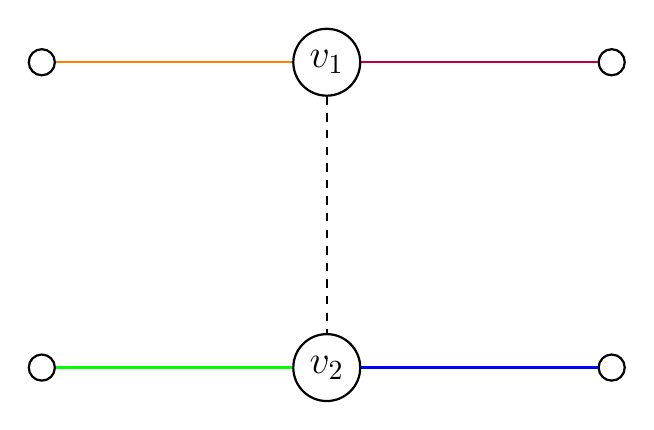
\begin{tikzpicture}[auto,node distance=3cm,
	thick,main node/.style={circle,draw,font=\sffamily\Large\bfseries}]
  	
    \node[main node] (1) {$v_1$};
    \node[main node] (2) [left = 3cm of 1]  {};
    \node[main node] (3) [right = 3cm of 1] {};
    \node[main node] (4) [below = 3cm of 1] {$v_2$};
    \node[main node] (5) [left = 3cm of 4] {}; {};
    \node[main node] (6) [right = 3cm of 4] {};] {};

    \path[draw,thick,draw=orange]
    (1) edge node {} (2)
    ;
    \path[draw,thick,draw=purple]
    (1) edge node {} (3)
    ;
    \path[draw,thick,draw=green]
    (4) edge node {} (5)
    ;
    \path[draw,thick,draw=blue]
    (4) edge node {} (6)
    ;
    \path[draw,thick,draw=black,dashed]
    (1) edge node {} (4)
    ;
	\end{tikzpicture}
\end{figure}


\section{Q 6.2.1}
	The $2n$ case:\\ Consider a $2n-1$ - gon with $2n^{th}$ vertex in the middle. 

	\begin{figure}[H]
	\centering
	\begin{tikzpicture}[auto,
	thick,main node/.style={circle,draw,font=\sffamily\Large\bfseries}]
  	
    \node[main node] (1) [label = $2n-2$]{};
    \node[main node] (2) [below right = 0.5cm and 2cm of 1,label = $2n-1$] {};
    \node[main node] (3) [below right = 1.5cm and 1.5cm of 2, label = $1$] {};
    \node[main node] (4) [below right = 2cm and 0.5cm of 3, label = $2$] {};
    \node[main node] (5) [below left = 9cm and 5cm of 1, label = below left:$n$]  {};
    \node[main node] (6) [below right = 1cm and 2cm of 5, label = below:$n-1$] {};
    \node[main node] (7) [above left = 2cm and 1cm of 5, label = left:$n+1$] {};
    \node[main node] (8) [below left = 5 cm and 1cm of 1, label = left:$2n$] {};

    \path[draw,thick, dashed]
    (1) edge node {} (2)
    (2) edge node {} (3)
    (3) edge node {} (4)
    (4) edge[bend left=55] node  {} (6)
    (5) edge node {} (6)
    (5) edge node {} (7)
    (7) edge[bend left=55] node  {} (1)
    (5) edge node {} (8)
    ;

	\end{tikzpicture}
\end{figure}

Matchings!\\

\begin{figure}[H]
	\centering
	\begin{tikzpicture}[auto,
	thick,main node/.style={circle,draw,font=\sffamily\Large\bfseries}]
  	
    \node[main node] (1) [label = $2n-2$]{};
    \node[main node] (2) [below right = 0.5cm and 2cm of 1,label = $2n-1$] {};
    \node[main node] (3) [below right = 1.5cm and 1.5cm of 2, label = $1$] {};
    \node[main node] (4) [below right = 2cm and 0.5cm of 3, label = $2$] {};
    \node[main node] (5) [below left = 9cm and 5cm of 1, label = below left:$n$]  {};
    \node[main node] (6) [below right = 1cm and 2cm of 5, label = below:$n-1$] {};
    \node[main node] (7) [above left = 2cm and 1cm of 5, label = left:$n+1$] {};
    \node[main node] (8) [below left = 5 cm and 1cm of 1, label = left:$2n$] {};

    \path[draw,thick, dashed]
    (1) edge node {} (2)
    (2) edge node {} (3)
    (3) edge node {} (4)
    (4) edge[bend left=55] node  {} (6)
    (5) edge node {} (6)
    (5) edge node {} (7)
    (7) edge[bend left=55] node  {} (1)
    (5) edge node {} (8)
    ;
        \path[draw,ultra thick, red]
    (1) edge node {} (4)
    (2) edge node {} (3)
    (6) edge node {} (7)
    (5) edge node {} (8)
    ;

	\end{tikzpicture}
\end{figure}

	The $2n-1$ case:\\ Now remove the middle vertex. We no longer have $2n-1$ perfect matchings, but we can still consider the problem in a similar fashion. We still consider the parallel matchings, except now we have an odd vertex in the polygon that is unsaturated. As we rotate the matchings around $2n-1$ times, I don't know what I"m saying waaaaaah.

	\begin{figure}[H]
	\centering
	\begin{tikzpicture}[auto,
	thick,main node/.style={circle,draw,font=\sffamily\Large\bfseries}]
  	
    \node[main node] (1) [label = $2n-2$]{};
    \node[main node] (2) [below right = 0.5cm and 2cm of 1,label = $2n-1$] {};
    \node[main node] (3) [below right = 1.5cm and 1.5cm of 2, label = $1$] {};
    \node[main node] (4) [below right = 2cm and 0.5cm of 3, label = $2$] {};
    \node[main node] (5) [below left = 9cm and 5cm of 1, label = below left:$n$]  {};
    \node[main node] (6) [below right = 1cm and 2cm of 5, label = below:$n-1$] {};
    \node[main node] (7) [above left = 2cm and 1cm of 5, label = left:$n+1$] {};


    \path[draw,thick, dashed]
    (1) edge node {} (2)
    (2) edge node {} (3)
    (3) edge node {} (4)
    (4) edge[bend left=55] node  {} (6)
    (5) edge node {} (6)
    (5) edge node {} (7)
    (7) edge[bend left=55] node  {} (1)
    ;
        \path[draw,ultra thick, red]
    (1) edge node {} (4)
    (2) edge node {} (3)
    (6) edge node {} (7)
    ;

	\end{tikzpicture}
\end{figure}

\section{Q 6.3.1}
	\begin{enumerate}[(a)]
	\item The number of periods needed in the week can be simply taken as $max\{\sum_i (p_{ij} , \sum_j (p_{ij}\}$. We then assume that we want an even distribution period across days and so divide this value by the number of days in the week, $5$.
	\item $\frac {\sum_{i,j} p_{ij}} {5 \times 8}$
	\end{enumerate}

\section{BONUS 6.2.6}
	\begin{enumerate}[(a)]
	\item Using Vizing's theorem (6.2) show that $\chi^\prime(G \times K_2) = \Delta(G \times K_2)$.\\
	It is immediately apparent that $\Delta(G \times K_2) = \Delta(G) + \Delta(K_2)$, in fact, this is clear for any two loopless graphs $\Delta(G \times H) = \Delta(G) + \Delta(H)$. We won't necessarily use that here, but it's good for intuition.\\
	$K_2$ is a simple stick - 2 vertices connected by an edge.\\
	Consider $G$ to be a graph with $V = {v_1,v_2,v_3}, E = {v_1v_2,v_2v_3}$, as below.\\

\begin{figure}[H]
	\centering
	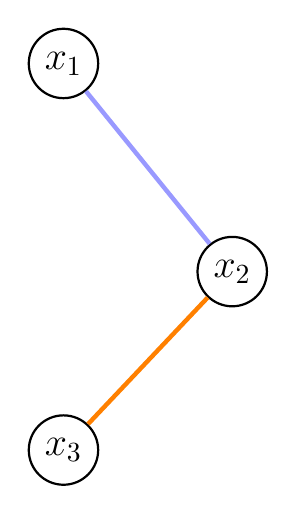
\begin{tikzpicture}[auto,
	thick,main node/.style={circle,draw,font=\sffamily\Large\bfseries}]
  	
    \node[main node] (1) {$x_1$};
    \node[main node] (2) [below right = 2cm and 1.5cm of 1]  {$x_2$};
    \node[main node] (3) [below = 4cm of 1] {$x_3$};

    \path[draw,ultra thick,blue!40]
    (1) edge node {} (2);
    \path[draw,ultra thick,orange]
    (2) edge node {} (3);
	\end{tikzpicture}
\end{figure}

And just there are no doubts as to what we're working with, here's $K_2$:

\begin{figure}[H]
	\centering
	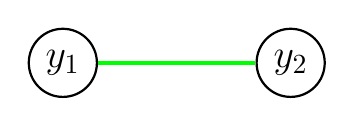
\begin{tikzpicture}[auto,
	thick,main node/.style={circle,draw,font=\sffamily\Large\bfseries}]
  	
    \node[main node] (1) {$y_1$};
    \node[main node] (2) [right = 2cm of 1]  {$y_2$};

    \path[draw,ultra thick,green]
    (1) edge node {} (2);
	\end{tikzpicture}
\end{figure}

	Now let's look at the product $G \times K_2$\\

\begin{figure}[H]
	\centering
	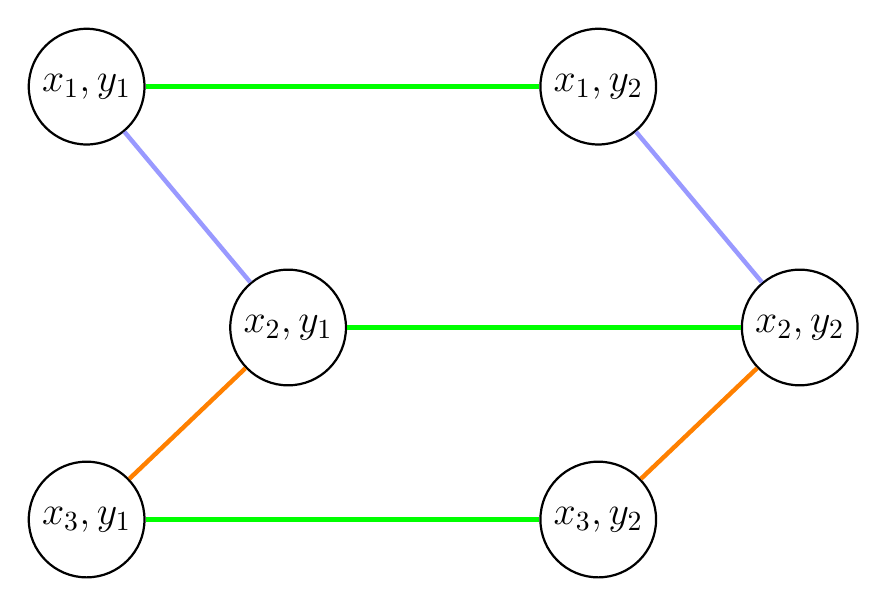
\begin{tikzpicture}[auto,
	thick,main node/.style={circle,draw,font=\sffamily\Large\bfseries}]
  	
    \node[main node] (1) {$x_1,y_1$};
    \node[main node] (2) [below right = 2cm and 1.5cm of 1]  {$x_2,y_1$};
    \node[main node] (3) [below = 4cm of 1] {$x_3,y_1$};

    \node[main node] (4) [right = 5cm of 1] {$x_1,y_2$};
    \node[main node] (5) [below right = 2cm and 1.5cm of 4] {$x_2,y_2$};
    \node[main node] (6) [below = 4cm of 4] {$x_3,y_2$};

    \path[draw,ultra thick,blue!40]
    (1) edge node {} (2)
    (4) edge node {} (5);
    
	\path[draw,ultra thick,orange]
    (2) edge node {} (3)
    (5) edge node {} (6);

    \path[draw,ultra thick,green]
    (1) edge node {} (4)
    (2) edge node {} (5)
    (3) edge node {} (6)
    ;

	\end{tikzpicture}
\end{figure}


	From (6.2) we know that for any loopless graph $G$ that we could choose, $\chi^\prime(G \times K_2) = \Delta(G \times K_2)$ or $\chi^\prime(G \times K_2) = \Delta(G \times K_2) + 1$. All we need to do is show that the $+ 1$ is unnecessary.\\

	\item Deduce that if $H$ is nontrivial with $\chi^\prime(H) = \Delta(H)$, then $\chi^\prime(G \times H) = \Delta(G \times H)$.\\

	\end{enumerate}



\end{document}
